%latex model.tex
%bibtex model
%latex model.tex
%latex model.tex
%pdflatex model.tex

%se poate lucra si online (de ex www.overleaf.com)


\documentclass[runningheads,a4paper,11pt]{report}

\usepackage{algorithmic}
\usepackage{algorithm} 
\usepackage{array}
\usepackage{amsmath}
\usepackage{amsfonts}
\usepackage{amssymb}
\usepackage{amsthm}
\usepackage{caption}
\usepackage{comment} 
\usepackage{epsfig} 
\usepackage{fancyhdr}
\usepackage[T1]{fontenc}
\usepackage{geometry} 
\usepackage{graphicx}
\usepackage[colorlinks]{hyperref} 
\usepackage[latin1]{inputenc}
\usepackage{multicol}
\usepackage{multirow} 
\usepackage{rotating}
\usepackage{setspace}
\usepackage{subfigure}
\usepackage{url}
\usepackage{verbatim}
\usepackage{xcolor}
\graphicspath{ {./images/} }

\pagestyle{fancy}
\fancyhf{}
\fancyhead[LE,RO]{ALL blood cell classification using federated learning}
\fancyfoot[RE,LO]{ITSG 2023-2024}
\fancyfoot[LE,RO]{\thepage}

\renewcommand{\headrulewidth}{2pt}
\renewcommand{\footrulewidth}{1pt}
\renewcommand{\headrule}{\hbox to\headwidth{%
  \color{lime}\leaders\hrule height \headrulewidth\hfill}}
\renewcommand{\footrule}{\hbox to\headwidth{%
  \color{lime}\leaders\hrule height \footrulewidth\hfill}}

\hypersetup{
pdftitle={artTitle},
pdfauthor={name},
pdfkeywords={pdf, latex, tex, ps2pdf, dvipdfm, pdflatex},
bookmarksnumbered,
pdfstartview={FitH},
urlcolor=cyan,
colorlinks=true,
linkcolor=red,
citecolor=green,
}


\setcounter{secnumdepth}{3}
\setcounter{tocdepth}{3}
\linespread{1}
\makeindex


\begin{document}

\begin{titlepage}
\sloppy

\begin{center}
BABE\c S BOLYAI UNIVERSITY, CLUJ NAPOCA, ROM\^ ANIA

FACULTY OF MATHEMATICS AND COMPUTER SCIENCE

\vspace{6cm}

\Huge \textbf{Acute Lymphoblastic Leukemia blood cell classification using federated learning}

\vspace{1cm}

\normalsize -- ITSG report --

\end{center}


\vspace{5cm}

\begin{flushright}
Muntean Andrei, Data Science, andrei.muntean@stud.ubbcluj.ro \\
Chiorean Alexandra, Data Science, maria.alexandra.chiorean@stud.ubbcluj.ro
\end{flushright}

\vspace{1cm}

\begin{center}
2023-2024
\end{center}

\end{titlepage}

\pagenumbering{gobble}

\begin{abstract}
	Text of abstract. Short info about: 
	\begin{itemize}
		\item project relevance/importance, 
		\item inteligent methods used for solving, 
		\item data involved in the numerical experiments; 
		\item conclude by the the results obtained.
		\item Please add a graphical abstract of your work. 
	\end{itemize}

\noindent
\textbf{\textcolor{green}{Remind that a good report should:}}
\begin{itemize}	
	\item be fun to read with many figures and visualizations;
	\item be easy to follow even for AI/ML novice;
	\item clearly convey the potential of AI/ML to the application domain;
	\item around 10 minutes to read (although this is not a hard constraint).
\end{itemize}

\end{abstract}


\tableofcontents

\newpage

\listoftables
\listoffigures
\listofalgorithms

\newpage

\setstretch{1.5}



\newpage

\pagenumbering{arabic}


 


\chapter{Introduction}
\label{chapter:introduction}

\section{What? Why? How?}
\label{section:what}

In US, approximately at each 3 minutes, a person is diagnosed with blood cancer. This disease is caused by the dysfunction of the bone marrow and can affect different blood types, resulting in different types of cancer like: Leukemia, lymphoma, myeloma, myelodysplastic syndromes (MDS), and myeloproliferative neoplasms (MPNs). In our project, we aim to reduce the diagnosis time by providing a computer based analysis of a microscopic image using an AI model. Moreover, to enable the model accuracy, we implement a federated learning approach, such that data does not leave the medical units.
\begin{itemize}
	\item What is the (scientific) problem? 
 Whenever it's the case for a cancer diagnosis, multiple doctors are called to give their professional opinion. The blood cell cancer is even more complex, most of the time needing different tests, which are also influenced by the stage of the cancer.  
	\item Why is it important? 
 Using peripheral blood smear (PBS) images, earlier detection of the ALL can be done, therefore more patients could be saved. Besides that, having a model that can predict the stage of the ALL, could help the doctors with a pragmatic opinion, obtaining a more precise and correct diagnosis for patients. The examination of these PBS images by laboratory users is riddled with problems such as diagnostic error because the non-specific nature of ALL signs and symptoms often leads to misdiagnosis.
	\item What is your basic approach? 
 The solution we proposed is based on a Convolutional Neural Network, which is known to obtain very accurate predictions on image tasks, having different architectures for classification tasks. In the medical field, patients confidence is really important, therefore datasets generation can be a very slow and bureaucratic. To avoid this impediment, we'll implement a federated learning approach that would speedup the entire process.
\end{itemize}

\textbf {A short discussion of how it fits into related work in the area is also desirable. Summarize the basic results and conclusions that you will present. }


\section{Paper structure and original contribution(s)}
\label{section:structure}

The research presented in this paper advances the theory, design, and implementation of several particular models. 

The main contribution of this report is to present an intelligent algorithm for solving the problem of blood cell cancer, concretely Acute Lymphoblastic Leukemia, which is very important since more and more patients are diagnosed with it. The algorithm is able to classify the blood samples in 4 classes: Benign, Pre-B, Pro-B, early Pre-B, all three being malign.

The second contribution of this report consists of building an intuitive, easy-to-use and user friendly software application. Our aim is to build a product that would enable doctors or patients to upload an image with the PBS on our website, where the model would predict the class of the blood sample. This application can be seen as a tool for doctors when they need a second, objective opinion, but also for the patients who could find a possible interpretation of their medical test before going to a specialist.

The third contribution in this report is related to the learning procedure. Since most of the medical data is very sensitive and confidential, we aim to train our model in a Federated Learning approach, making the development and accuracy of the algorithm increase sooner. The data that the medical units is already having we'll be fed to the model, encoded, such that the data cannot be retrieved from the model. In this way, we take advantage of the quality and quantity of data, that each unit has, but it reaches to a greater purpose where patients from different location can be helped, on click away.

\textbf{The present work contains $xyz$ bibliographical references and is structured in five chapters as follows.}

The first chapter is a short introduction in the blood cell cancer classification and its purpose in the current medical context.

The second chapter describes the problem in more details, having also more information about the design decision taken for implementing the software application.

The chapter \ref{chapter:stateOfArt} details briefly presents the current state of the art algorithms in both medical image classification and federated learning approaches.

The chapter \ref{chapter:proposedApproach} details the solution we are going to implement, starting from a smaller model, on which more complex layers we'll be added later. Moreover, this section will detail the necessary changes and adaptations done in order to synchronise model's learning results.

In the chapter \ref{chapter:application} an analytical analysis will be drawn. Result obtain during the training process and a comparison with SOTA, and also describing the methodology of obtaining them should be documented.

Chapter \ref{chapter:swot} will describe the strengths, the opportunities, threads and weaknesses of our algorithm, as well as of our software application.

Finally, a conclusion chapter will be summarizing our results, future plans, why and how our approach is helping the society around us.



\chapter{Scientific Problem}
\label{section:scientificProblem}


\section{Problem definition}
\label{section:problemDefinition}

Blood cell cancers, also known as hematologic cancers primarily affect the blood, bone marrow, lymph nodes, and spleen. These cancers are classified based on the specific type of blood cell affected and whether they are acute (develop rapidly) or chronic (develop gradually). Our main focus is to identify if a patient suffers from a benign or malign  Acute Lymphoblastic Leukemia (ALL) which affects immature lymphocytes. To do this we are using a CNN which  can analyze vast amounts of medical images, to detect subtle patterns indicative of early-stage ALL. Early diagnosis often leads to more effective treatments and improved outcomes. 

CNNs excel at recognizing intricate patterns within images, even subtle ones that might be challenging for the human eye to discern. In PBS images, CNNs can identify specific cell types, anomalies, and morphological features. They can efficiently process large datasets, including thousands of PBS images, in a relatively short amount of time. This ability is essential for quick and accurate diagnosis, especially in busy clinical settings. CNNs can undergo continuous learning with new data, allowing them to adapt and improve their performance over time. As more annotated PBS images become available, CNNs can refine their algorithms, leading to enhanced accuracy in diagnosis.

However, while CNNs can outperform doctors in specific tasks related to PBS image analysis, it's important to note that these technologies are most effective when used in conjunction with medical professionals. Doctors can provide critical context, interpret complex clinical situations, and make informed decisions based on the combined analysis of imaging data, patient history, and other relevant information. The synergy between intelligent algorithms and medical expertise can lead to the most accurate and comprehensive diagnoses.

Training such a model can become a very challenging task, due to the data sensitivity. Even though hospitals are possessing it, the collecting process can be very complicate. A solution for this problem is the federated learning. This method addresses privacy concerns, allowing institutions to collaborate without sharing sensitive patient data. Local devices train models on their data, sending only model updates to a central server, reducing communication overhead and ensuring data security.

As mention before, our CNN model has an PBS image as input and it returns 4 probabilities, each for the classes available: benign, Pre-B, early Pre-B and Pro-B. The class with the heights probability, will be the result for the processed sample. The image is uploaded in our web-base application and the result is shown there, after the inference on the model is done.



\chapter{State of the art/Related work}
\label{chapter:stateOfArt}

The application development is enabled by TensorFlow, a machine learning framework which provides the backbone for building intricate neural networks and implementing the CNN model, framework that is build upon Python, a versatile and widely-used programming language. 

On the application side we use Django, a high-level Python web framework, which excels in the creation of robust and scalable web applications, providing a structured, efficient approach to backend development. 

Last but not least, we use Docker, for the federated learning process, which ensures consistency and portability, encapsulating the entire application and its dependencies within containers.

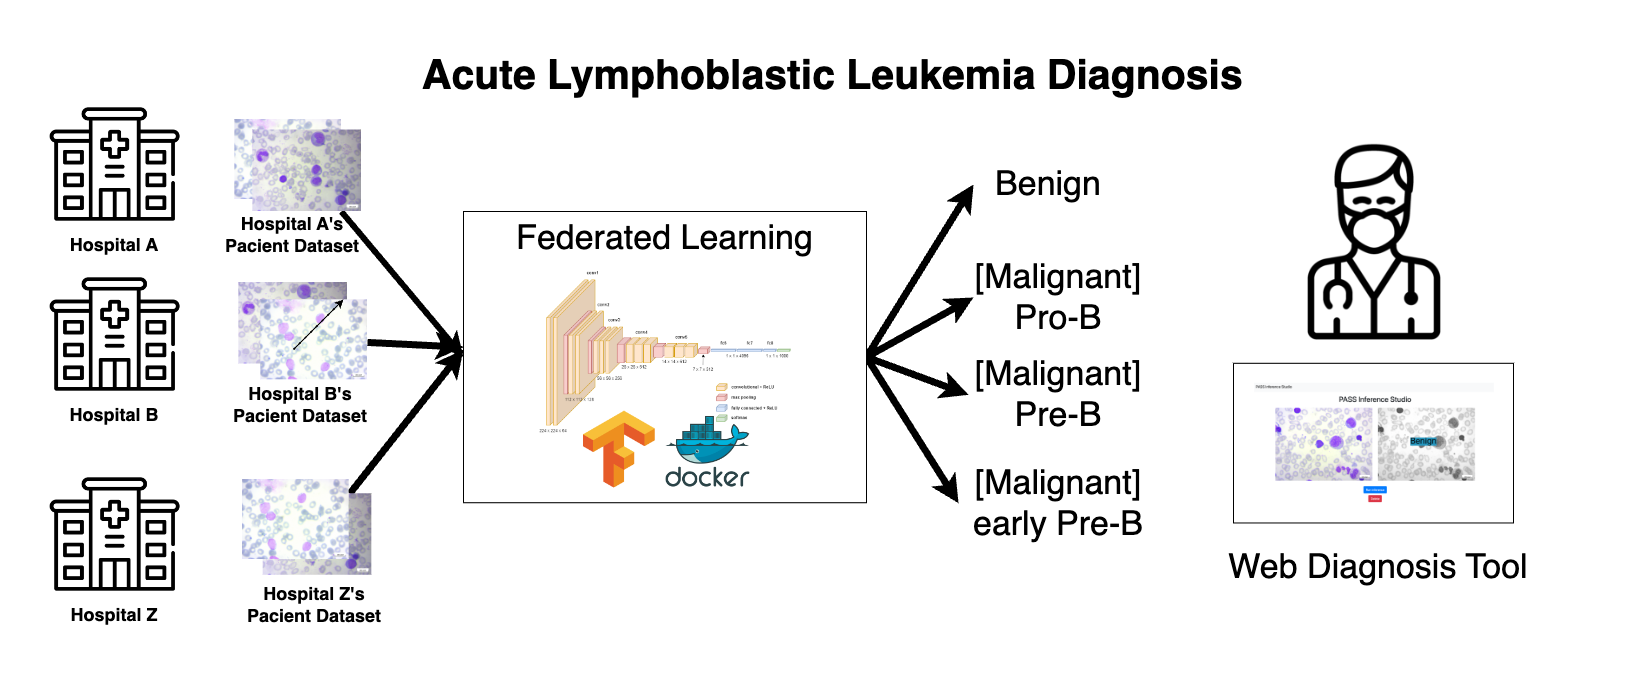
\includegraphics[scale=0.25]{images/diagram.png}


\chapter{Investigated approach}
\label{chapter:proposedApproach}

Describe your approach!

Describe in reasonable detail the algorithm you are using to address this problem. A psuedocode description of the algorithm you are using is frequently useful. Trace through a concrete example, showing how your algorithm processes this example. The example should be complex enough to illustrate all of the important aspects of the problem but simple enough to be easily understood. If possible, an intuitively meaningful example is better than one with meaningless symbols.

\section{Convolutional Neural Networks}

Convolutional Neural Networks, are a class of deep learning models specifically designed for processing images and videos. They are widely used in computer vision tasks like image recognition, object detection, and image generation. 

CNNs are able to automatically learn and extract hierarchical features from the input data. This is achieved through convolutional layers, which apply convolution operations to the input, enabling the network to detect patterns like edges, corners, and textures, making CNN very effective in medical image processing. These convolutional operations are followed by activation functions like ReLU (Rectified Linear Unit) to introduce non-linearity into the model.

\section{CNN architectures used for solving the ALL blood cell classification}
\subsection{MobileNetV2}

MobileNetV2 is an advanced deep learning architecture specifically optimized for on-device vision applications, particularly well-suited for mobile and edge devices. Developed by Google researchers, it represents an evolution of the original MobileNet model, focusing on enhancing both accuracy and efficiency in computer vision tasks.

MobileNetV2 introduces innovative features such as inverted residuals with linear bottlenecks, enabling improved gradient flow during training and maximizing computational resources. Its design includes a lightweight depthwise separable convolution followed by a linear (1x1) convolution, capturing complex patterns efficiently within a limited computational budget. Inverted residuals allow for efficient feature reuse across different layers, while depthwise separable convolutions significantly reduce parameters and computations. The model also incorporates width and resolution multipliers, offering flexibility to balance accuracy and computational efficiency. 

MobileNetV2 finds widespread application in real-time tasks like image recognition, object detection, and scene analysis on mobile devices due to its lightweight nature, making it ideal for resource-constrained environments.
\begin{figure}[h]
    \centering
    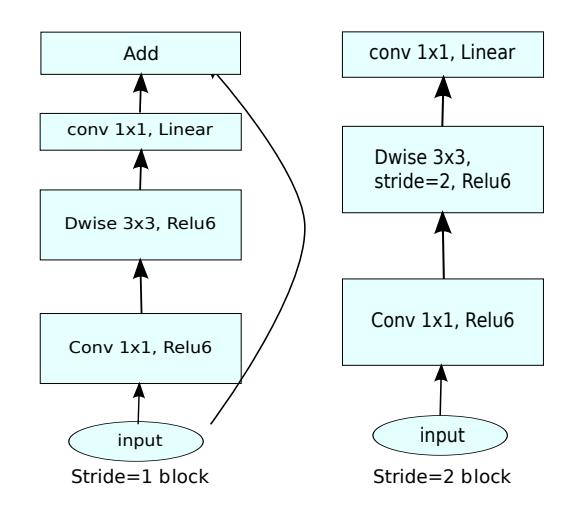
\includegraphics[scale=0.5]{images/mobilenetv2.png} 
    \caption{MobileNetV2 blocks }
\end{figure}

This backbone has approximately 3.4 million trainable parameters with 53 deep layers.
\subsection{EfficientNetB0}

EfficientNetB0 is the foundational model in the EfficientNet family of convolutional neural network architectures, known for its remarkable balance between accuracy and computational efficiency. Developed by Google researchers, this model leverages compound scaling to ensure that network depth, width, and resolution grow proportionally, leading to superior performance without a significant increase in computational demands. It incorporates depthwise separable convolutions for reduced parameter count and computational overhead, making it well-suited for resource-constrained devices. Regularization techniques such as dropout and batch normalization enhance its generalization and training speed. EfficientNetB0 is widely applied in various computer vision tasks, including image classification, object detection, and segmentation, and is a preferred choice for projects that require a combination of high accuracy and efficient model design.

The EfficientNetB0 has 11 million trainable parameters.

\subsection{MobileNet Tiny}

MobileNet Tiny serves as the third choice for our classification task backbone, introduced in response to the suboptimal performance of federated learning models. Derived from the groundwork laid by SSD-Lite and MobileNetV2, MobileNet-Tiny is designed to enable real-time object detection on non-GPU computers and edge devices, such as Raspberry Pi, addressing the need for efficient processing in resource-constrained environments.

\begin{figure}[h]
    \centering
    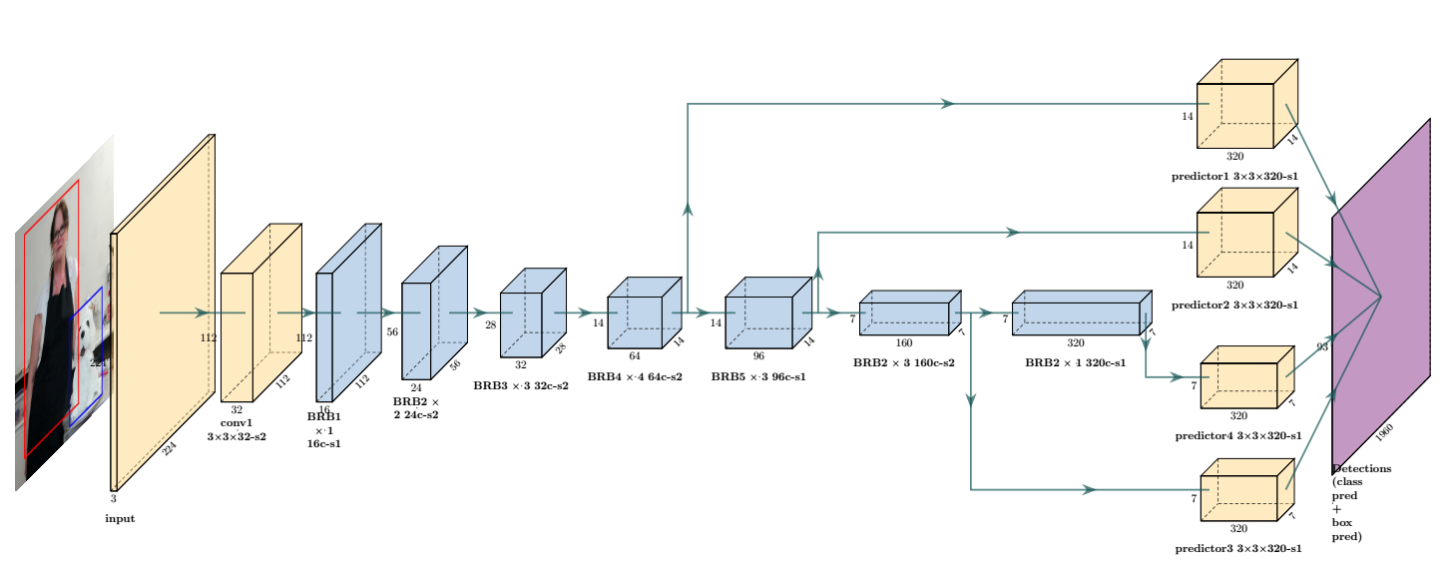
\includegraphics[scale=0.5]{images/tiny.png} 
    \caption{Tiny MobileNet}
\end{figure}

\section{Deep Learning on Decentralized Data}
Since our application processes medical data, it has a very strong privacy requirement: The patients’ data should not leave the hospital. To deal with this issue, we implement a Federated Learning approach. This enables our intelligent algorithm to learn collaboratively from multiple hospitals (edge devices) without ever sharing the sensitive data between them or with a central server. The process can be described in four phases. In the first phase, the server starts with a central model. The edge devices improve the model with their own data in phase two. In phase three, only the updates to the models are sent to the server.  Finally, the server combines the received models into a single model. The process repeats for multiple iterations which are usually just referred to as rounds.

As we have an image classification task, we will need to train a CNN in a federated way. This can pose a challenge as commonly used image classification models are quite large. We don’t expect edge devices to be very powerful, so we need to make the training process as efficient as possible. Our solution for this problem is to combine Federated Learning with Transfer Learning, meaning that we take one of the already trained image classification models (see the section above) and we freeze the backbone of the network. That means that we will only need to train the head of the network. (which we replace with a new head that can classify between our four classes). In this way we drastically reduce the number of parameters that our model has.

The development of a Federated Learning based application requires two steps: the experimentation and the deployment. In the following paragraphs we will only focus on experimentation. To experiment with federated learning, we use the dataset from Kaggle and we split it into multiple smaller datasets, one for each client. We keep this data in a different folder and we load it into a different Tensorflow Dataset, as each one of these datasets is associated with a client id. We also take into consideration that this split does not have to be equal, as in the real world some hospitals will have more data and others will have less data.

After we have split the original dataset for each client, we define the model. We use MobileNetV2 with the frozen backbone. At this step we have the model and the data, therefore we can start the federated learning simulation. For doing that, we need to initialise the weighted federated averaging algorithm. It is weighted because different weights are assigned to each client update. This is useful for giving more importance to some clients than others. To initialise this federated learning algorithm, we have to provide two optimizers. While regular training only requires a single optimizer, for federated learning we have to have two optimizers, one for the clients and one for the server.

Once the federated learning algorithm has been initialised, we can start the federated learning simulation. The simulation consists of multiple rounds, as explained in the first paragraph of this section. The steps are repeated for a predefined number of rounds. After the proof-of-concept has been established using the simulation, we move to the real world and try to achieve the same thing using docker. With docker compose, we define the number of clients and we mount to each client a different dataset folder. That means that now we have our data logically separated between clients, and we can test the concept in a real environment.


\chapter{Application (numerical validation)}
\label{chapter:application}


Explain the experimental methodology and the numerical results obtained with your approach and the state of art approache(s).

Try to perform a comparison of several approaches.

Statistical validation of the results.


\section{Methodology}
\label{section:methodology}

\begin{itemize}
	\item What are criteria you are using to evaluate your method? 
	\item What specific hypotheses does your experiment test? Describe the experimental methodology that you used. 
	\item What are the dependent and independent variables? 
	\item What is the training/test data that was used, and why is it realistic or interesting? Exactly what performance data did you collect and how are you presenting and analyzing it? Comparisons to competing methods that address the same problem are particularly useful.
\end{itemize}

\section{Data}
\label{section:data}

Describe the used data.

\section{Results}
\label{section:results}

Present the quantitative results of your experiments. Graphical data presentation such as graphs and histograms are frequently better than tables. What are the basic differences revealed in the data. Are they statistically significant?

\section{Discussion}
\label{section:discussion}

\begin{itemize}
	\item Is your hypothesis supported? 
	\item What conclusions do the results support about the strengths and weaknesses of your method compared to other methods? 
	\item How can the results be explained in terms of the underlying properties of the algorithm and/or the data. 
\end{itemize}


\chapter{SWOT Analysis}
\label{chapter:swot}


\chapter{Conclusion and future work}
\label{chapter:concl}

Try to emphasise the strengths and the weaknesses of your approach.
What are the major shortcomings of your current method? For each shortcoming, propose additions or enhancements that would help overcome it. 

Briefly summarize the important results and conclusions presented in the paper. 

\begin{itemize}
	\item What are the most important points illustrated by your work? 
	\item How will your results improve future research and applications in the area? 
\end{itemize}


\chapter{Latex examples}

Item example: 

\begin{itemize}
	\item content of item1
 	\item content of item2
 	\item content of item3
\end{itemize}



Figure example 

$\ldots$ (see Figure \ref{swarmsize})

\begin{figure}[htbp]
	\centerline{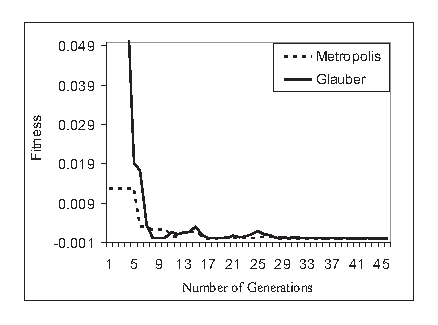
\includegraphics{Fig/FitEvol.eps}}  
	\caption{The evolution of the swarm size during the GA generations. This results were obtained for the $f_2$ test function with 5 dimensions.}
	\label{swarmsize}
\end{figure}


Table example: (see Table \ref{tab3PSO})


\begin{table}[htbp]
	\caption{The parameters of the PSO algorithm (the micro level algorithm) used to compute the fitness of a GA chromosome.}
	\label{tab3PSO}
		\begin{center}
			\begin{tabular}{p{220pt}c}

				\textbf{Parameter}& \textbf{Value} \\
				\hline\hline
 				Number of generations& 50 \\
 				Number of function evaluations/generation& 10 \\
 				Number of dimensions of the function to be optimized& 5 \\
 				Learning factor $c_{1}$& 2 \\
 				Learning factor $c_{2}$ & 1.8\\
 				Inertia weight& 0.5 + $\frac{rand()}{2}$\\
		
			\end{tabular}
		\end{center}
\end{table}

Algorithm example 

$\ldots$ (see Algorithm \ref{NGalg}).


\algsetup{indent=1em, linenosize=\footnotesize}

\begin{algorithm}
	\caption{SGA - Spin based Genetic AQlgorithm}
	\label{NGalg}
		\begin{algorithmic}


			\STATE \textbf{BEGIN}
  		\STATE @ Randomly create the initial GA population.
  		\STATE @ Compute the fitness of each individual.
  		\FOR{i=1 TO NoOfGenerations}
  			\FOR{j=1 TO PopulationSize}
  				\STATE p $\leftarrow$ RandomlySelectParticleFromGrid();
  				\STATE n $\leftarrow$ RandomlySelectParticleFromNeighbors(p);
  				\STATE @ Crossover(p, n, off);
  				\STATE @ Compute energy $\Delta H$
  				\IF {$\Delta H$ satisfy the Ising condition}
  					\STATE @ Replace(p,off);
  				\ENDIF
  			\ENDFOR
  		\ENDFOR
  		\STATE \textbf{END}
\end{algorithmic}
\end{algorithm}


\bibliographystyle{plain}
\bibliography{BibAll}

\end{document}

